\documentclass[11pt,a4paper]{uebung}

\usepackage[british]{babel}
\usepackage{epsfig}
\usepackage{rotate}
\usepackage{amsmath,amsthm,amssymb}
\usepackage{color}
\makeatletter\let\@amsfonts=P\makeatother
\usepackage{graphicx}
\usepackage{typearea}
\usepackage{multicol}
\usepackage{amsfonts}
\usepackage[nounderscore]{syntax}
\usepackage{enumitem}
\newcommand{\comment}[1]{\marginpar{\small{\bf Comment:} #1}}

\usepackage{tikz}
\usetikzlibrary{shapes,arrows,backgrounds,%
matrix,patterns,arrows,decorations.pathmorphing,decorations.pathreplacing,%
positioning,fit,calc,decorations.text,shadows%
}

\newcommand{\solution}[1]{\par {\bf Solution:}\\#1}



%put your Matrikelnummer here instead of the XXXXXXXX
% if your group has less than 3 members, just delete the remaining XXXXXXXX
\newcommand\matrikelnummerA[0]{XXXXXXXX}
\newcommand\matrikelnummerB[0]{XXXXXXXX}
\newcommand\matrikelnummerC[0]{XXXXXXXX}
%put your Matrikelnummer here instead of the XXXXXXXX



\def\cT{\mathcal{T}}


\begin{document}
\newcommand{\Vorlesung}{Formal Methods in Computer Science}
\newcommand{\Semester}{SS 2012}
\newcommand{\Prof}{Uwe Egly}
\newcommand{\AssisA}{Antonius Weinzierl}
\newcommand{\AssisB}{}

%%%%%%%%%%%%%%%%%%%%%%%%%%%%%%%%%%%%%%%%%%%%%%%%%%%%%%%%%%%%%%%%%%%%%%%%%%%%%%

\Uebungsblatt{2 (10 points)}{
  \begin{tabular}{rl}
   Matrikelnummer(n): &\matrikelnummerA \\
   &\matrikelnummerB \\
   &\matrikelnummerC
  \end{tabular}
}

%%%%%%%%%%%%%%%%%%%%%%%%%%%%%%%%%%%%%%%%%%%%%%%%%%%%%%%%%%%%%%%%%%%%%%%%%%%%%%


\Aufgabe[Tseitin Transformation \hfill \bf (0.5 + 1 + 1.5 points)]

\begin{enumerate}
\item Extend Tseitin's transformation for the connectives $\leftrightarrow$
  (equivalence) and $\oplus$ (XOR). Find the necessary clauses for the new schemes
  $l_i \leftrightarrow (l_{i'} \leftrightarrow l_{i''})$ and $l_k
  \leftrightarrow (l_{k'} \oplus l_{k''})$.
  
  \solution{
  }

\item Apply Tseitin's transformation to the following formula $\psi$: $a \rightarrow
  \big( b \lor \neg (a \leftrightarrow c)\big)$.
  
  Hint: You do not need to introduce labels for propositions $a,b,$ and $c$.
  \solution{
  }

\item Let $\psi$ be a propositional formula and $D^\psi$ the set of clauses
  resulting from Tseitin's transformation on $\psi$. Prove that the following
  holds:
  
  \centerline{If $\psi$ is satisfiable then $D^\psi$ is satisfiable.}

  You only need to prove this for the connectives $\land$ and $\neg$.
  %\lor,\neg, \rightarrow$.
  Use the below clause schemes, which introduce a new label for every boolean
  variable.
  \begin{align*}
    L_a \leftrightarrow a && (\neg L_a \lor a)&& (L_a \lor \neg a)\\
    L_\phi \leftrightarrow (L_1 \land L_2) && (\neg L_\phi \lor L_1)&& (\neg
    L_\phi \lor L_2)&& (L_\phi \lor \neg L_1 \lor \neg L_2)\\
    L_\phi \leftrightarrow \neg L_1 && (\neg L_\phi \lor \neg L_1)&& (L_\phi
    \lor L_1)
  \end{align*}
  
  \solution{
  }
\end{enumerate}


%%%%%%%%%%%%%%%%%%%%%%%%%%%%%%%%%%%%%%%%%%%%%%%%%%%%%%%%%%%%%%%%%%%%%%%%%%%%%%

\newpage
\Aufgabe[Implication Graphs \hfill \bf (2+1+1.5 points)]
\begin{enumerate}
\item Let $\mathcal{D}$ be the following set of clauses:
  \begin{align*}
    c_1:& (A \lor B)\\
    c_2:& (A \lor G \lor H)\\
    c_3:& (\neg B \lor \neg D \lor E)\\
    c_4:& (E \lor F)\\
    c_5:& (\neg F \lor \neg G \lor D)\\
    c_6:& (\neg C \lor G \lor J)\\
    c_7:& (\neg J \lor \neg H)
  \end{align*}
  Draw the implication graph resulting from $\mathcal{D}$ with decisions
  $A=0@1$, $C=1@2$, $E=0@3$. Find the first UIP, and learn a new clause using
  the first-UIP scheme (use resolution).

  \solution{
  }

\item Prove that in a conflict graph the first UIP is uniquely defined, i.e.,
  prove that there is exactly one node in the graph which is a first UIP.

  \solution{
  }

\item Let $\mathcal{C}$ be a set of clauses and $G$ a conflict graph with
  respect to $\mathcal{C}$. Prove: if a clause $C_l$ is learned following the
  first-UIP scheme, then $C_l$ is a consequence of $\mathcal{C}$.

  \solution{
  }
\end{enumerate}


%%%%%%%%%%%%%%%%%%%%%%%%%%%%%%%%%%%%%%%%%%%%%%%%%%%%%%%%%%%%%%%%%%%%%%%%%%%%%%

\newpage
\Aufgabe[Sparse Method \hfill \bf (1.5 points)]
Apply the Sparse Method including preprocessing on the formula $\varphi^E$
below to obtain a propositional formula.
\begin{displaymath}
  (x_1 \neq x_2 \lor x_2=x_3 ) \land \big[ (x_2 \neq x_4 \land x_3=x_4
  \land x_4=x_5)
  \lor (x_6 \neq x_5 \land x_6=x_7 \land x_7=x_3)\big]
\end{displaymath}

  \solution{
We define the above formula as $\varphi^{E}$. We use the Sparse Method to compute  an equisatisfiable formula in propostional logic.
We begin to seperate the formula in equality literals $E_{=}$ and inequality literals $E_{\neq}$. 
\bigskip

$E_{=} = \{x_2 = x_3, x_3 = x_4 , x_4 = x_5 , x_6 = x_7, x_7 =x_3 \}$

\bigskip

$E_{\neq} =\{x_1 \neq x_2, x_2 \neq x_4 , x_6 \neq x_5 \} $

Now we construct the corresponding equality graph $G^{E} (\varphi^{E} )$ :

 \begin{figure}[h]
    \centering
    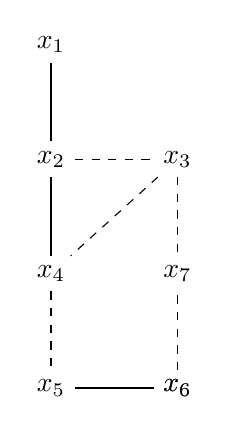
\begin{tikzpicture}
      \node(x1){$x_1$};
      \node[below=of x1](x2){$x_2$};
      \node[right=of x2](x3){$x_3$};
      \node[below=of x2](x4){$x_4$};  
      \node[below=of x4](x5){$x_5$};
      \node[right=of x5](x6){$x_6$};
      \node[below=of x3](x7){$x_7$};
      \node[below=of x7](x6){$x_6$};
      
      
      \draw[] (x1) -- (x2);
      \draw[dashed] (x2) -- (x3);
      \draw[dashed] (x3) -- (x4); 
      \draw[dashed] (x3) -- (x7);
      \draw[] (x2) -- (x4);
      \draw[dashed] (x4) -- (x5);
      \draw[] (x5) -- (x6);
      \draw[dashed] (x6) -- (x7);
 
    \end{tikzpicture}
    \caption{$G^E(\varphi^E)$, dashed lines represent equality, solid lines disequality.}
    \label{fig:sp1}
  \end{figure}

  }

Now we have to search for contradictory cycle. This are cycles which have exactly one dis-equality edge.
Only the Edge $(x_1,x_2)$ are not part of a simple contradictory cycle, therefore we set those edges to $true$ in $\varphi^E$
and obtain $\varphi^E_2$ as:

 \begin{displaymath}
    [ (true \lor  x_2 = x_3 ) \land \big[ (x_2 \neq x_4 \land x_3=x_4
  \land x_4=x_5)
  \lor (x_6 \neq x_5 \land x_6=x_7 \land x_7=x_3)\big]
 \end{displaymath}

  Propositional simplification of $\varphi^E_2$ leads to :
 
 \begin{displaymath}
   \big[ (x_2 \neq x_4 \land x_3=x_4
  \land x_4=x_5)
  \lor (x_6 \neq x_5 \land x_6=x_7 \land x_7=x_3)\big]
 \end{displaymath}

Now we construct the new corresponding equality graph $G^{E} (\varphi^{E_2} )$ :

 \begin{figure}[h]
    \centering
    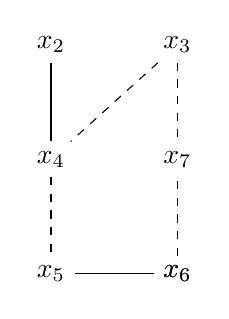
\begin{tikzpicture}
      \node(x2){$x_2$};
      \node[right=of x2](x3){$x_3$};
      \node[below=of x2](x4){$x_4$};  
      \node[below=of x4](x5){$x_5$};
      \node[right=of x5](x6){$x_6$};
      \node[below=of x3](x7){$x_7$};
      \node[below=of x7](x6){$x_6$};
      
      
      \draw[dashed] (x3) -- (x4); 
      \draw[dashed] (x3) -- (x7);
      \draw[] (x2) -- (x4);
      \draw[dashed] (x4) -- (x5);
      \draw[] (x5) -- (x6);
      \draw[dashed] (x6) -- (x7);
 
    \end{tikzpicture}
    \caption{$G^E(\varphi^E_2)$, dashed lines represent equality, solid lines disequality.}
    \label{fig:sp2}
  \end{figure}

\bigskip

Now we have to search again for contradictory cycle.
The Edge $(x_2)$ is not part of a simple contradictory cycle, therefore we set those edges to $true$ in $\varphi^E_2$
and obtain $\varphi^E_3$ as:

\begin{displaymath}
   \big[ (TRUE \land x_3=x_4 \land x_4=x_5)
  \lor (x_6 \neq x_5 \land x_6=x_7 \land x_7=x_3)\big]
 \end{displaymath}
 

  Propositional simplification of $\varphi^E_3$ leads to :
 
 \begin{displaymath}
   \big[ ( x_3=x_4
  \land x_4=x_5)
  \lor (x_6 \neq x_5 \land x_6=x_7 \land x_7=x_3)\big]
 \end{displaymath}


Now are no more nodes not part of a contradictory cycle. So we can build the e propositional skeleton $ e(\varphi^E_3) $ by
  relabeling the equality literals with $e_{i,j}$.


\begin{displaymath}
   \big[ ( e_{3,7} \land e_{4,5} )
  \lor ( \neg e_{6,5} \land e_{6,7} \land e_{7,3})\big]
 \end{displaymath}

The next step is to create a nonpolar version of the graph. To ensure that there are no hidden computational complexity we make the new graph chordal. To do so we have to add some edges at the corresponding nodes like $(x_7,x_5)$ and $(x_3,x_5)$. There are also others possibilities to make the graph chordal. If a graph is chordal then each cycles has the length 3. 

\begin{figure}[h]
    \centering
    \begin{tikzpicture}
      \node(x3){$x_3$};
      \node[left=of x3](x4){$x_4$};  
      \node[below=of x4](x5){$x_5$};
      \node[below=of x3](x7){$x_7$};
      \node[below=of x7](x6){$x_6$};
      
      
      \draw[] (x3) -- (x4); 
      \draw[] (x3) -- (x7);
      \draw[] (x2) -- (x4);
      \draw[] (x4) -- (x5);
      \draw[] (x5) -- (x6);
      \draw[] (x6) -- (x7);
 
    \end{tikzpicture}
    \caption{Non-chordal graph}
    \label{fig:sp3}
  \end{figure}


\begin{figure}[h]
    \centering
    \begin{tikzpicture}
      \node(x3){$x_3$};
      \node[left=of x3](x4){$x_4$};  
      \node[below=of x4](x5){$x_5$};
      \node[below=of x3](x7){$x_7$};
      \node[below=of x7](x6){$x_6$};
      
      
      \draw[] (x3) -- (x4);
      \draw[] (x3) -- (x5);
      \draw[] (x5) -- (x7);
      \draw[] (x3) -- (x7);
      \draw[] (x2) -- (x4);
      \draw[] (x4) -- (x5);
      \draw[] (x5) -- (x6);
      \draw[] (x6) -- (x7);
 
    \end{tikzpicture}
    \caption{Chordal graph}
    \label{fig:sp4}
  \end{figure}

At last we have to derive according transitivity constraints for each triangle to obtain $B_t$.
  
\begin{eqnarray*}
    B_t:= &(e_{3,7} \land e_{3,5} \rightarrow e_{7,5}) \land
   (e_{3,7} \land e_{7,5} \rightarrow e_{3,5}) \land
    (e_{3,5} \land e_{5,7} \rightarrow e_{5,8}) \land & \quad \quad \text{for }\triangle
    (x_3,x_5,x_7)\\
    %
    &(e_{3,4} \land e_{4,5} \rightarrow e_{3,5}) \land
    (e_{4,5} \land e_{3,5} \rightarrow e_{3,4}) \land
    (e_{3,4} \land e_{3,5} \rightarrow e_{4,5}) \land & \quad \quad \text{for
    } \triangle (x_3,x_4,x_5)\\
    %
    &(e_{5,7} \land e_{5,6} \rightarrow e_{6,7}) \land
    (e_{5,7} \land e_{6,7} \rightarrow e_{5,6}) \land
    (e_{5,6} \land e_{6,7} \rightarrow e_{5,7}) &\quad \quad\text{for }  \triangle (x_7,x_5,x_8)
  \end{eqnarray*}

  The sparse Methode generates at the final form  $e(\varphi^E_3) \land B_t$.

  

%%%%%%%%%%%%%%%%%%%%%%%%%%%%%%%%%%%%%%%%%%%%%%%%%%%%%%%%%%%%%%%%%%%%%%%%%%%%%%

\newpage
\Aufgabe[Ackermann's Reduction \hfill \bf (1 point)]
Apply Ackermann's reduction on the following EUF-formula $\varphi$ to obtain
an EU formula:
\begin{displaymath}
  f\left(f\left(g\left(a\right),b\right),a\right) = f(g(a),b) \rightarrow \big[ f(x,y) = g(f(g(a),b)) \land
  g(f(a,y))=d \big]
\end{displaymath}


\solution{
  The first step of the ackermann´s reduction enummerate each variable from outside to inside and from left to right. 
 
 \begin{displaymath}
  f_4\left(f_1\left(g_1\left(a\right),b\right),a\right) = f_1(g_1(a),b) \rightarrow \big[ f_2(x,y) = g_2(f_1(g(a),b)) \land
   g_3(f_3(a,y))=d \big]
 \end{displaymath}

After the enummeration ....

  


}


\end{document}
